% =========================================================
% Chapter 4 - Functional Requirements and Use Case Specifications
% Project: AITasker
%
% Yêu cầu trong main.tex:
% \usepackage{graphicx}
% \usepackage{float}
% \usepackage{longtable}
% \usepackage{array}
% \usepackage{booktabs}
% \graphicspath{{figures/}}
%
% Tên hình được sử dụng đúng theo thư mục figures:
%   Usecase.png
% =========================================================

\chapter{Yêu cầu chức năng và đặc tả Use Case}
\label{chap:functional-requirements}

\section{Giới thiệu}
\label{sec:chapter4-introduction}

Chương này trình bày các yêu cầu chức năng của hệ thống AITasker và đặc tả chi tiết các Use Case chính. Nội dung được xây dựng dựa trên phạm vi nghiệp vụ, sơ đồ Use Case tổng quát, Activity Diagram, Sequence Diagram, State Diagram và mô hình dữ liệu của hệ thống.

Mỗi yêu cầu chức năng được định danh theo mẫu \textbf{FR-xxx}. Mỗi Use Case được định danh theo mẫu \textbf{UC-xx}. Các quy tắc nghiệp vụ được định danh theo mẫu \textbf{BR-xxx}, trong khi các quy tắc kiểm tra dữ liệu sử dụng mẫu \textbf{VR-xxx}.

\section{Tác nhân hệ thống}
\label{sec:actors}

\begin{longtable}{|p{2.2cm}|p{3.6cm}|p{8.0cm}|}
\caption{Danh sách tác nhân của hệ thống AITasker}
\label{tab:actors} \\ \hline
\textbf{Mã} & \textbf{Tác nhân} & \textbf{Mô tả} \\ \hline
\endfirsthead
\hline
\textbf{Mã} & \textbf{Tác nhân} & \textbf{Mô tả} \\ \hline
\endhead

ACT-01 & Khách truy cập & Người dùng chưa đăng nhập, có thể xem thông tin công khai, đăng ký tài khoản và đăng nhập. \\ \hline
ACT-02 & Doanh nghiệp & Người dùng đăng dự án, quản lý proposal, thuê chuyên gia, quản lý hợp đồng, milestone, thanh toán và đánh giá. \\ \hline
ACT-03 & Chuyên gia AI & Người cung cấp dịch vụ AI, quản lý hồ sơ, tìm kiếm dự án, gửi proposal, thực hiện milestone và nhận đánh giá. \\ \hline
ACT-04 & Quản trị viên & Người quản lý tài khoản, danh mục, dự án, hợp đồng, nội dung và báo cáo thống kê. \\ \hline
ACT-05 & Cổng thanh toán & Dịch vụ bên ngoài xử lý giao dịch thanh toán hoặc hoàn tiền. \\ \hline
ACT-06 & Dịch vụ Email & Dịch vụ bên ngoài gửi email xác thực, khôi phục mật khẩu và thông báo. \\ \hline
ACT-07 & Dịch vụ lưu trữ & Dịch vụ bên ngoài lưu avatar, CV, portfolio và tệp đính kèm dự án. \\ \hline
\end{longtable}

\section{Sơ đồ Use Case tổng quát}
\label{sec:usecase-overview}

Sơ đồ Use Case tổng quát mô tả các chức năng mà từng tác nhân có thể thực hiện trong hệ thống AITasker.

\begin{figure}[H]
    \centering
    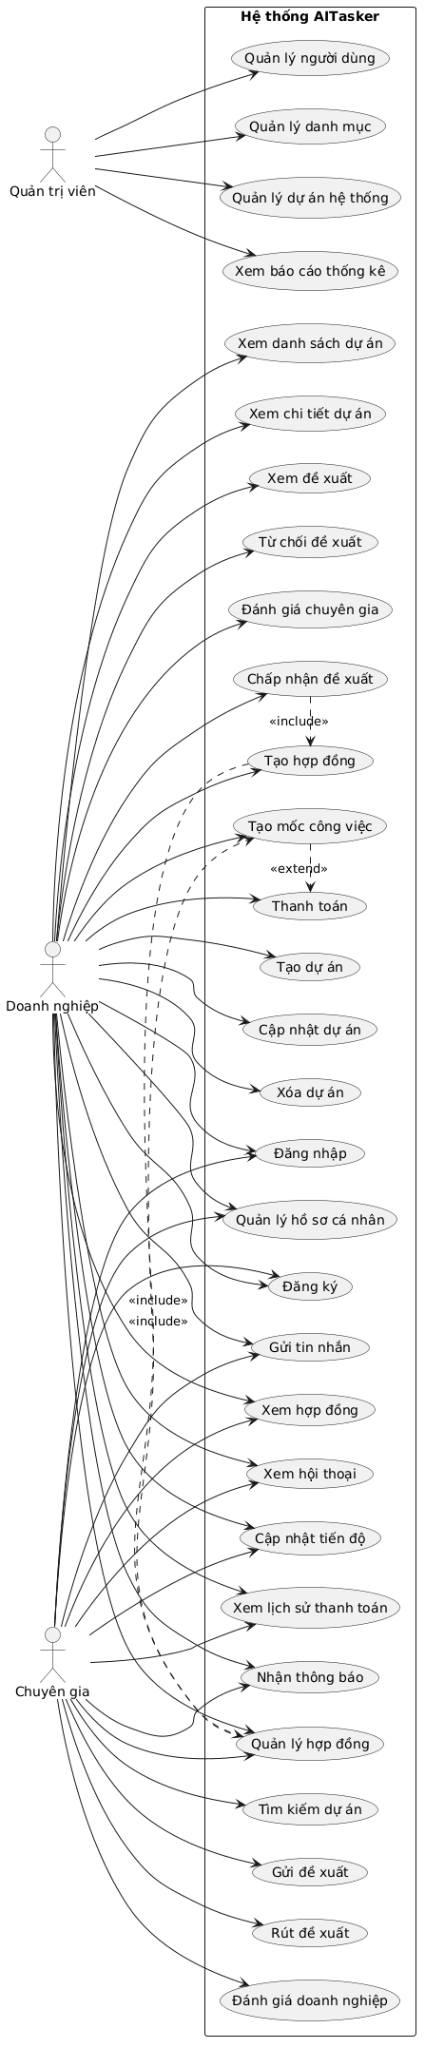
\includegraphics[height=0.88\textheight,keepaspectratio]{Usecase.png}
    \caption{Sơ đồ Use Case tổng quát của hệ thống AITasker}
    \label{fig:usecase-overview}
\end{figure}

Từ Hình~\ref{fig:usecase-overview}, có thể thấy ba nhóm người dùng chính có phạm vi chức năng khác nhau:

\begin{itemize}
    \item Quản trị viên quản lý người dùng, danh mục, dự án hệ thống và báo cáo thống kê.
    \item Doanh nghiệp tạo dự án, xem proposal, thuê chuyên gia, quản lý hợp đồng, milestone, thanh toán và đánh giá chuyên gia.
    \item Chuyên gia AI tìm kiếm dự án, gửi hoặc rút proposal, quản lý hợp đồng, cập nhật tiến độ và đánh giá doanh nghiệp.
\end{itemize}

\section{Danh sách yêu cầu chức năng}
\label{sec:functional-requirements-list}

\subsection{Nhóm xác thực và tài khoản}

\begin{longtable}{|p{2.0cm}|p{4.2cm}|p{7.6cm}|}
\caption{Yêu cầu chức năng nhóm xác thực và tài khoản}
\label{tab:fr-authentication} \\ \hline
\textbf{Mã} & \textbf{Tên yêu cầu} & \textbf{Mô tả} \\ \hline
\endfirsthead
\hline
\textbf{Mã} & \textbf{Tên yêu cầu} & \textbf{Mô tả} \\ \hline
\endhead

FR-001 & Đăng ký tài khoản & Hệ thống cho phép khách truy cập đăng ký tài khoản doanh nghiệp hoặc chuyên gia bằng email và mật khẩu. \\ \hline
FR-002 & Đăng nhập & Hệ thống xác thực email và mật khẩu, sau đó cấp JWT cho người dùng hợp lệ. \\ \hline
FR-003 & Đăng xuất & Hệ thống cho phép người dùng kết thúc phiên đăng nhập hiện tại. \\ \hline
FR-004 & Quên mật khẩu & Hệ thống tạo token đặt lại mật khẩu và gửi đường dẫn qua email. \\ \hline
FR-005 & Đổi mật khẩu & Người dùng đã đăng nhập có thể thay đổi mật khẩu sau khi xác nhận mật khẩu hiện tại. \\ \hline
FR-006 & Xem hồ sơ & Người dùng có thể xem thông tin hồ sơ của chính mình. \\ \hline
FR-007 & Cập nhật hồ sơ & Người dùng có thể cập nhật thông tin cá nhân hoặc tổ chức. \\ \hline
FR-008 & Tải ảnh đại diện & Người dùng có thể tải lên hoặc thay đổi ảnh đại diện. \\ \hline
FR-009 & Phân quyền truy cập & Hệ thống giới hạn chức năng theo vai trò doanh nghiệp, chuyên gia và quản trị viên. \\ \hline
FR-010 & Quản lý trạng thái tài khoản & Admin có thể khóa hoặc mở khóa tài khoản người dùng. \\ \hline
\end{longtable}

\subsection{Nhóm hồ sơ doanh nghiệp và chuyên gia}

\begin{longtable}{|p{2.0cm}|p{4.2cm}|p{7.6cm}|}
\caption{Yêu cầu chức năng nhóm hồ sơ}
\label{tab:fr-profile} \\ \hline
\textbf{Mã} & \textbf{Tên yêu cầu} & \textbf{Mô tả} \\ \hline
\endfirsthead
\hline
\textbf{Mã} & \textbf{Tên yêu cầu} & \textbf{Mô tả} \\ \hline
\endhead

FR-011 & Quản lý hồ sơ doanh nghiệp & Doanh nghiệp có thể cập nhật tên công ty, mô tả, địa chỉ, website và thông tin liên hệ. \\ \hline
FR-012 & Quản lý hồ sơ chuyên gia & Chuyên gia có thể cập nhật họ tên, chức danh, tiểu sử, vị trí, kinh nghiệm và mức giá theo giờ. \\ \hline
FR-013 & Quản lý kỹ năng & Chuyên gia có thể thêm hoặc xóa kỹ năng chuyên môn. \\ \hline
FR-014 & Quản lý CV và portfolio & Chuyên gia có thể tải lên CV, portfolio và tài liệu chứng minh năng lực. \\ \hline
FR-015 & Tìm kiếm chuyên gia & Doanh nghiệp có thể tìm kiếm chuyên gia theo tên, kỹ năng, vị trí, rating và mức giá. \\ \hline
FR-016 & Xem hồ sơ chuyên gia & Người dùng có thể xem thông tin công khai, kỹ năng, kinh nghiệm và điểm đánh giá của chuyên gia. \\ \hline
\end{longtable}

\subsection{Nhóm quản lý dự án}

\begin{longtable}{|p{2.0cm}|p{4.2cm}|p{7.6cm}|}
\caption{Yêu cầu chức năng nhóm quản lý dự án}
\label{tab:fr-project} \\ \hline
\textbf{Mã} & \textbf{Tên yêu cầu} & \textbf{Mô tả} \\ \hline
\endfirsthead
\hline
\textbf{Mã} & \textbf{Tên yêu cầu} & \textbf{Mô tả} \\ \hline
\endhead

FR-017 & Tạo dự án & Doanh nghiệp có thể tạo dự án với tiêu đề, mô tả, ngân sách, thời hạn và danh mục. \\ \hline
FR-018 & Cập nhật dự án & Doanh nghiệp có thể chỉnh sửa dự án khi dự án chưa bắt đầu thực hiện. \\ \hline
FR-019 & Xóa hoặc hủy dự án & Doanh nghiệp có thể xóa hoặc hủy dự án nếu chưa có hợp đồng đang hoạt động. \\ \hline
FR-020 & Xem danh sách dự án & Người dùng có thể xem danh sách dự án phù hợp với quyền truy cập. \\ \hline
FR-021 & Xem chi tiết dự án & Người dùng có thể xem thông tin chi tiết của một dự án. \\ \hline
FR-022 & Tìm kiếm và lọc dự án & Chuyên gia có thể tìm dự án theo từ khóa, danh mục, ngân sách, trạng thái và thời hạn. \\ \hline
FR-023 & Đính kèm tài liệu dự án & Doanh nghiệp có thể tải lên tài liệu yêu cầu hoặc dữ liệu mẫu cho dự án. \\ \hline
FR-024 & Quản lý trạng thái dự án & Hệ thống cập nhật trạng thái dự án theo vòng đời: OPEN, IN\_PROGRESS, COMPLETED, CLOSED hoặc CANCELLED. \\ \hline
\end{longtable}

\subsection{Nhóm quản lý Proposal}

\begin{longtable}{|p{2.0cm}|p{4.2cm}|p{7.6cm}|}
\caption{Yêu cầu chức năng nhóm quản lý Proposal}
\label{tab:fr-proposal} \\ \hline
\textbf{Mã} & \textbf{Tên yêu cầu} & \textbf{Mô tả} \\ \hline
\endfirsthead
\hline
\textbf{Mã} & \textbf{Tên yêu cầu} & \textbf{Mô tả} \\ \hline
\endhead

FR-025 & Gửi proposal & Chuyên gia có thể gửi đề xuất cho dự án đang mở. \\ \hline
FR-026 & Cập nhật proposal & Chuyên gia có thể chỉnh sửa proposal khi proposal còn ở trạng thái PENDING. \\ \hline
FR-027 & Rút proposal & Chuyên gia có thể rút proposal trước khi doanh nghiệp chấp nhận. \\ \hline
FR-028 & Xem danh sách proposal & Doanh nghiệp có thể xem các proposal của dự án do mình sở hữu. \\ \hline
FR-029 & Xem chi tiết proposal & Doanh nghiệp có thể xem chi phí, thời gian và thư giới thiệu của từng proposal. \\ \hline
FR-030 & Chấp nhận proposal & Doanh nghiệp có thể chọn một proposal phù hợp để thuê chuyên gia. \\ \hline
FR-031 & Từ chối proposal & Doanh nghiệp có thể từ chối proposal không phù hợp. \\ \hline
FR-032 & Quản lý trạng thái proposal & Hệ thống quản lý các trạng thái PENDING, ACCEPTED, REJECTED và WITHDRAWN. \\ \hline
\end{longtable}

\subsection{Nhóm hợp đồng và milestone}

\begin{longtable}{|p{2.0cm}|p{4.2cm}|p{7.6cm}|}
\caption{Yêu cầu chức năng nhóm hợp đồng và milestone}
\label{tab:fr-contract} \\ \hline
\textbf{Mã} & \textbf{Tên yêu cầu} & \textbf{Mô tả} \\ \hline
\endfirsthead
\hline
\textbf{Mã} & \textbf{Tên yêu cầu} & \textbf{Mô tả} \\ \hline
\endhead

FR-033 & Tạo hợp đồng & Hệ thống tự động tạo hợp đồng khi doanh nghiệp chấp nhận proposal. \\ \hline
FR-034 & Xem hợp đồng & Doanh nghiệp và chuyên gia có thể xem hợp đồng mà họ tham gia. \\ \hline
FR-035 & Cập nhật hợp đồng & Thông tin được phép có thể được cập nhật theo quyền và trạng thái hợp đồng. \\ \hline
FR-036 & Chấm dứt hợp đồng & Hợp đồng có thể bị chấm dứt theo quy tắc nghiệp vụ. \\ \hline
FR-037 & Tạo milestone & Doanh nghiệp có thể chia hợp đồng thành các mốc công việc. \\ \hline
FR-038 & Cập nhật milestone & Chuyên gia có thể cập nhật tiến độ và kết quả thực hiện milestone. \\ \hline
FR-039 & Nghiệm thu milestone & Doanh nghiệp có thể xác nhận milestone đã hoàn thành. \\ \hline
FR-040 & Quản lý trạng thái hợp đồng & Hệ thống quản lý ACTIVE, COMPLETED, TERMINATED và DISPUTED. \\ \hline
FR-041 & Quản lý trạng thái milestone & Hệ thống quản lý PENDING, IN\_PROGRESS, SUBMITTED, REVISION\_REQUIRED, DONE, PAID hoặc CANCELLED tùy phạm vi hiện thực. \\ \hline
\end{longtable}

\subsection{Nhóm thanh toán}

\begin{longtable}{|p{2.0cm}|p{4.2cm}|p{7.6cm}|}
\caption{Yêu cầu chức năng nhóm thanh toán}
\label{tab:fr-payment} \\ \hline
\textbf{Mã} & \textbf{Tên yêu cầu} & \textbf{Mô tả} \\ \hline
\endfirsthead
\hline
\textbf{Mã} & \textbf{Tên yêu cầu} & \textbf{Mô tả} \\ \hline
\endhead

FR-042 & Tạo yêu cầu thanh toán & Doanh nghiệp có thể tạo giao dịch thanh toán cho milestone đủ điều kiện. \\ \hline
FR-043 & Xử lý thanh toán & Hệ thống chuyển yêu cầu đến cổng thanh toán và tiếp nhận kết quả. \\ \hline
FR-044 & Ghi nhận giao dịch & Hệ thống lưu mã giao dịch, số tiền, thời gian, phương thức và trạng thái thanh toán. \\ \hline
FR-045 & Xem lịch sử thanh toán & Doanh nghiệp và chuyên gia có thể xem giao dịch liên quan đến hợp đồng. \\ \hline
FR-046 & Hoàn tiền & Hệ thống có thể xử lý hoàn tiền theo quy định và quyền quản trị. \\ \hline
FR-047 & Quản lý trạng thái thanh toán & Hệ thống quản lý PENDING, PROCESSING, PAID, FAILED, REFUNDED hoặc CANCELLED tùy phạm vi tích hợp. \\ \hline
\end{longtable}

\subsection{Nhóm trao đổi, thông báo và đánh giá}

\begin{longtable}{|p{2.0cm}|p{4.2cm}|p{7.6cm}|}
\caption{Yêu cầu chức năng nhóm trao đổi, thông báo và đánh giá}
\label{tab:fr-communication} \\ \hline
\textbf{Mã} & \textbf{Tên yêu cầu} & \textbf{Mô tả} \\ \hline
\endfirsthead
\hline
\textbf{Mã} & \textbf{Tên yêu cầu} & \textbf{Mô tả} \\ \hline
\endhead

FR-048 & Tạo hội thoại & Hệ thống tạo hội thoại giữa doanh nghiệp và chuyên gia khi proposal được chấp nhận hoặc hợp đồng được tạo. \\ \hline
FR-049 & Gửi tin nhắn & Người tham gia hội thoại có thể gửi và nhận tin nhắn. \\ \hline
FR-050 & Xem hội thoại & Người dùng có thể xem lịch sử tin nhắn của hội thoại mà mình tham gia. \\ \hline
FR-051 & Nhận thông báo & Người dùng nhận thông báo khi có proposal, hợp đồng, milestone, thanh toán hoặc đánh giá mới. \\ \hline
FR-052 & Quản lý thông báo & Người dùng có thể xem danh sách thông báo và đánh dấu đã đọc. \\ \hline
FR-053 & Tạo đánh giá & Doanh nghiệp và chuyên gia có thể đánh giá bên còn lại khi hợp đồng đã hoàn thành. \\ \hline
FR-054 & Cập nhật điểm trung bình & Hệ thống tính lại điểm đánh giá trung bình sau khi có review hợp lệ. \\ \hline
FR-055 & Quản lý review & Admin có thể ẩn hoặc xóa review vi phạm nếu chức năng này được triển khai. \\ \hline
\end{longtable}

\subsection{Nhóm quản trị và thống kê}

\begin{longtable}{|p{2.0cm}|p{4.2cm}|p{7.6cm}|}
\caption{Yêu cầu chức năng nhóm quản trị và thống kê}
\label{tab:fr-administration} \\ \hline
\textbf{Mã} & \textbf{Tên yêu cầu} & \textbf{Mô tả} \\ \hline
\endfirsthead
\hline
\textbf{Mã} & \textbf{Tên yêu cầu} & \textbf{Mô tả} \\ \hline
\endhead

FR-056 & Quản lý người dùng & Admin có thể xem, tìm kiếm, cập nhật trạng thái, khóa hoặc mở khóa tài khoản. \\ \hline
FR-057 & Quản lý danh mục & Admin có thể tạo, cập nhật và xóa danh mục dự án. \\ \hline
FR-058 & Quản lý dự án hệ thống & Admin có thể theo dõi và xử lý dự án vi phạm. \\ \hline
FR-059 & Quản lý hợp đồng & Admin có thể xem và hỗ trợ xử lý hợp đồng có vấn đề. \\ \hline
FR-060 & Xem dashboard & Người dùng có thể xem dashboard phù hợp với vai trò. \\ \hline
FR-061 & Xem thống kê & Admin có thể xem số lượng người dùng, dự án, proposal, hợp đồng, giao dịch và doanh thu. \\ \hline
\end{longtable}

\section{Đặc tả Use Case chi tiết}
\label{sec:usecase-specifications}

\subsection{UC-01: Đăng nhập}

\begin{longtable}{|p{3.5cm}|p{10.2cm}|}
\hline
\textbf{Thuộc tính} & \textbf{Nội dung} \\ \hline
Mã Use Case & UC-01 \\ \hline
Tên Use Case & Đăng nhập \\ \hline
Tác nhân & Doanh nghiệp, Chuyên gia AI, Quản trị viên \\ \hline
Mô tả & Người dùng đăng nhập bằng email và mật khẩu để truy cập chức năng theo vai trò. \\ \hline
Tiền điều kiện & Người dùng đã có tài khoản và tài khoản không bị khóa. \\ \hline
Kích hoạt & Người dùng chọn chức năng đăng nhập. \\ \hline
Luồng chính &
1. Hệ thống hiển thị biểu mẫu đăng nhập.\newline
2. Người dùng nhập email và mật khẩu.\newline
3. Người dùng nhấn nút đăng nhập.\newline
4. Hệ thống kiểm tra dữ liệu đầu vào.\newline
5. Hệ thống tìm tài khoản theo email.\newline
6. Hệ thống xác minh mật khẩu bằng BCrypt.\newline
7. Hệ thống kiểm tra trạng thái tài khoản.\newline
8. Hệ thống tạo JWT.\newline
9. Hệ thống chuyển người dùng đến dashboard phù hợp. \\ \hline
Luồng thay thế &
A1. Thiếu trường bắt buộc: hệ thống hiển thị lỗi.\newline
A2. Email không tồn tại: hệ thống thông báo tài khoản không tồn tại.\newline
A3. Mật khẩu sai: hệ thống thông báo đăng nhập thất bại.\newline
A4. Tài khoản bị khóa: hệ thống từ chối đăng nhập. \\ \hline
Hậu điều kiện & Người dùng có phiên đăng nhập hợp lệ và được cấp quyền theo vai trò. \\ \hline
Yêu cầu liên quan & FR-002, FR-009 \\ \hline
\end{longtable}

\subsection{UC-02: Đăng ký tài khoản}

\begin{longtable}{|p{3.5cm}|p{10.2cm}|}
\hline
\textbf{Thuộc tính} & \textbf{Nội dung} \\ \hline
Mã Use Case & UC-02 \\ \hline
Tên Use Case & Đăng ký tài khoản \\ \hline
Tác nhân & Khách truy cập \\ \hline
Mô tả & Khách truy cập tạo tài khoản doanh nghiệp hoặc chuyên gia AI. \\ \hline
Tiền điều kiện & Email chưa được sử dụng trong hệ thống. \\ \hline
Kích hoạt & Người dùng chọn chức năng đăng ký. \\ \hline
Luồng chính &
1. Hệ thống hiển thị biểu mẫu đăng ký.\newline
2. Người dùng chọn loại tài khoản.\newline
3. Người dùng nhập thông tin bắt buộc.\newline
4. Hệ thống kiểm tra dữ liệu.\newline
5. Hệ thống băm mật khẩu.\newline
6. Hệ thống tạo User và hồ sơ tương ứng.\newline
7. Hệ thống thông báo đăng ký thành công. \\ \hline
Luồng thay thế &
A1. Email đã tồn tại: hệ thống yêu cầu dùng email khác.\newline
A2. Mật khẩu không đạt yêu cầu: hệ thống hiển thị quy tắc mật khẩu.\newline
A3. Xác nhận mật khẩu không khớp: hệ thống từ chối tạo tài khoản. \\ \hline
Hậu điều kiện & Tài khoản và hồ sơ người dùng được lưu trong cơ sở dữ liệu. \\ \hline
Yêu cầu liên quan & FR-001, FR-009 \\ \hline
\end{longtable}

\subsection{UC-03: Tạo dự án}

\begin{longtable}{|p{3.5cm}|p{10.2cm}|}
\hline
\textbf{Thuộc tính} & \textbf{Nội dung} \\ \hline
Mã Use Case & UC-03 \\ \hline
Tên Use Case & Tạo dự án \\ \hline
Tác nhân & Doanh nghiệp \\ \hline
Mô tả & Doanh nghiệp tạo dự án AI mới để nhận proposal từ chuyên gia. \\ \hline
Tiền điều kiện & Doanh nghiệp đã đăng nhập và có hồ sơ hợp lệ. \\ \hline
Kích hoạt & Doanh nghiệp chọn nút tạo dự án. \\ \hline
Luồng chính &
1. Hệ thống hiển thị biểu mẫu tạo dự án.\newline
2. Doanh nghiệp nhập tiêu đề, mô tả, danh mục, ngân sách và deadline.\newline
3. Doanh nghiệp tải tệp đính kèm nếu cần.\newline
4. Hệ thống kiểm tra dữ liệu.\newline
5. Hệ thống lưu dự án với trạng thái OPEN.\newline
6. Hệ thống lưu tệp đính kèm nếu có.\newline
7. Hệ thống thông báo tạo dự án thành công. \\ \hline
Luồng thay thế &
A1. Thiếu trường bắt buộc: hiển thị lỗi.\newline
A2. Ngân sách không hợp lệ: yêu cầu nhập lại.\newline
A3. Deadline không hợp lệ: từ chối lưu.\newline
A4. Tệp sai định dạng hoặc quá kích thước: từ chối tải lên. \\ \hline
Hậu điều kiện & Dự án được tạo và hiển thị trong danh sách dự án đang mở. \\ \hline
Yêu cầu liên quan & FR-017, FR-023, FR-024 \\ \hline
\end{longtable}

\subsection{UC-04: Tìm kiếm dự án}

\begin{longtable}{|p{3.5cm}|p{10.2cm}|}
\hline
\textbf{Thuộc tính} & \textbf{Nội dung} \\ \hline
Mã Use Case & UC-04 \\ \hline
Tên Use Case & Tìm kiếm dự án \\ \hline
Tác nhân & Chuyên gia AI \\ \hline
Mô tả & Chuyên gia tìm dự án phù hợp theo từ khóa và bộ lọc. \\ \hline
Tiền điều kiện & Chuyên gia có quyền truy cập danh sách dự án. \\ \hline
Kích hoạt & Chuyên gia nhập từ khóa hoặc chọn bộ lọc. \\ \hline
Luồng chính &
1. Hệ thống hiển thị danh sách dự án.\newline
2. Chuyên gia nhập từ khóa hoặc bộ lọc.\newline
3. Hệ thống truy vấn dự án phù hợp.\newline
4. Hệ thống hiển thị kết quả.\newline
5. Chuyên gia chọn dự án để xem chi tiết. \\ \hline
Luồng thay thế & Không có dự án phù hợp: hệ thống hiển thị danh sách rỗng và gợi ý thay đổi bộ lọc. \\ \hline
Hậu điều kiện & Chuyên gia xem được kết quả tìm kiếm hoặc chi tiết dự án. \\ \hline
Yêu cầu liên quan & FR-020, FR-021, FR-022 \\ \hline
\end{longtable}

\subsection{UC-05: Gửi Proposal}

\begin{longtable}{|p{3.5cm}|p{10.2cm}|}
\hline
\textbf{Thuộc tính} & \textbf{Nội dung} \\ \hline
Mã Use Case & UC-05 \\ \hline
Tên Use Case & Gửi Proposal \\ \hline
Tác nhân & Chuyên gia AI \\ \hline
Mô tả & Chuyên gia gửi đề xuất thực hiện một dự án đang mở. \\ \hline
Tiền điều kiện & Chuyên gia đã đăng nhập; dự án OPEN; chuyên gia chưa gửi proposal cho dự án. \\ \hline
Kích hoạt & Chuyên gia chọn chức năng gửi proposal. \\ \hline
Luồng chính &
1. Hệ thống hiển thị biểu mẫu proposal.\newline
2. Chuyên gia nhập giá đề xuất, thời gian thực hiện và thư giới thiệu.\newline
3. Chuyên gia nhấn gửi proposal.\newline
4. Hệ thống kiểm tra dự án và proposal đã tồn tại.\newline
5. Hệ thống kiểm tra dữ liệu.\newline
6. Hệ thống lưu proposal với trạng thái PENDING.\newline
7. Hệ thống gửi thông báo cho doanh nghiệp. \\ \hline
Luồng thay thế &
A1. Dự án không còn OPEN: hệ thống từ chối.\newline
A2. Chuyên gia đã gửi proposal: hệ thống không cho tạo thêm.\newline
A3. Dữ liệu không hợp lệ: hệ thống hiển thị lỗi. \\ \hline
Hậu điều kiện & Proposal được lưu và xuất hiện trong danh sách proposal của dự án. \\ \hline
Yêu cầu liên quan & FR-025, FR-032, FR-051 \\ \hline
\end{longtable}

\subsection{UC-06: Chấp nhận Proposal và thuê chuyên gia}

\begin{longtable}{|p{3.5cm}|p{10.2cm}|}
\hline
\textbf{Thuộc tính} & \textbf{Nội dung} \\ \hline
Mã Use Case & UC-06 \\ \hline
Tên Use Case & Chấp nhận Proposal và thuê chuyên gia \\ \hline
Tác nhân & Doanh nghiệp \\ \hline
Mô tả & Doanh nghiệp chấp nhận một proposal và hệ thống tạo hợp đồng. \\ \hline
Tiền điều kiện & Proposal PENDING; dự án chưa có hợp đồng ACTIVE. \\ \hline
Kích hoạt & Doanh nghiệp chọn proposal và nhấn chấp nhận. \\ \hline
Luồng chính &
1. Hệ thống hiển thị thông tin proposal.\newline
2. Doanh nghiệp xác nhận lựa chọn.\newline
3. Hệ thống kiểm tra proposal và dự án.\newline
4. Hệ thống cập nhật proposal được chọn thành ACCEPTED.\newline
5. Hệ thống cập nhật các proposal còn lại thành REJECTED.\newline
6. Hệ thống tạo Contract ở trạng thái ACTIVE.\newline
7. Hệ thống chuyển Project sang IN\_PROGRESS.\newline
8. Hệ thống tạo Conversation.\newline
9. Hệ thống gửi thông báo cho chuyên gia. \\ \hline
Luồng thay thế &
A1. Proposal không hợp lệ hoặc không còn PENDING: hệ thống từ chối.\newline
A2. Dự án đã có hợp đồng ACTIVE: hệ thống không tạo thêm.\newline
A3. Lỗi trong transaction: hệ thống rollback toàn bộ thay đổi. \\ \hline
Hậu điều kiện & Hợp đồng ACTIVE được tạo giữa doanh nghiệp và chuyên gia. \\ \hline
Yêu cầu liên quan & FR-030, FR-031, FR-033, FR-048, FR-051 \\ \hline
\end{longtable}

\subsection{UC-07: Quản lý Milestone}

\begin{longtable}{|p{3.5cm}|p{10.2cm}|}
\hline
\textbf{Thuộc tính} & \textbf{Nội dung} \\ \hline
Mã Use Case & UC-07 \\ \hline
Tên Use Case & Quản lý Milestone \\ \hline
Tác nhân & Doanh nghiệp, Chuyên gia AI \\ \hline
Mô tả & Doanh nghiệp tạo milestone, chuyên gia cập nhật tiến độ và doanh nghiệp nghiệm thu. \\ \hline
Tiền điều kiện & Hợp đồng ở trạng thái ACTIVE. \\ \hline
Kích hoạt & Một bên truy cập danh sách milestone của hợp đồng. \\ \hline
Luồng chính &
1. Doanh nghiệp tạo milestone với tiêu đề, mô tả, số tiền và deadline.\newline
2. Hệ thống lưu milestone ở trạng thái PENDING.\newline
3. Chuyên gia bắt đầu thực hiện và chuyển sang IN\_PROGRESS.\newline
4. Chuyên gia gửi kết quả.\newline
5. Doanh nghiệp kiểm tra kết quả.\newline
6. Doanh nghiệp nghiệm thu.\newline
7. Hệ thống chuyển milestone sang DONE. \\ \hline
Luồng thay thế &
A1. Hợp đồng không ACTIVE: hệ thống từ chối thao tác.\newline
A2. Doanh nghiệp yêu cầu chỉnh sửa: milestone chuyển sang REVISION\_REQUIRED hoặc IN\_PROGRESS.\newline
A3. Milestone bị hủy: chuyển sang CANCELLED. \\ \hline
Hậu điều kiện & Milestone được cập nhật và đủ điều kiện thanh toán nếu ở trạng thái DONE. \\ \hline
Yêu cầu liên quan & FR-037, FR-038, FR-039, FR-041 \\ \hline
\end{longtable}

\subsection{UC-08: Thanh toán Milestone}

\begin{longtable}{|p{3.5cm}|p{10.2cm}|}
\hline
\textbf{Thuộc tính} & \textbf{Nội dung} \\ \hline
Mã Use Case & UC-08 \\ \hline
Tên Use Case & Thanh toán Milestone \\ \hline
Tác nhân & Doanh nghiệp, Cổng thanh toán \\ \hline
Mô tả & Doanh nghiệp thanh toán cho milestone đã hoàn thành. \\ \hline
Tiền điều kiện & Hợp đồng ACTIVE; milestone DONE; milestone chưa được thanh toán. \\ \hline
Kích hoạt & Doanh nghiệp chọn chức năng thanh toán. \\ \hline
Luồng chính &
1. Hệ thống hiển thị thông tin thanh toán.\newline
2. Doanh nghiệp chọn phương thức thanh toán.\newline
3. Hệ thống tạo Payment ở trạng thái PENDING.\newline
4. Hệ thống gửi yêu cầu đến cổng thanh toán.\newline
5. Cổng thanh toán xử lý giao dịch.\newline
6. Cổng thanh toán trả kết quả thành công.\newline
7. Hệ thống cập nhật Payment thành PAID.\newline
8. Hệ thống kiểm tra các milestone còn lại.\newline
9. Hệ thống cập nhật Contract thành COMPLETED nếu tất cả đã hoàn thành và được thanh toán.\newline
10. Hệ thống gửi thông báo cho các bên. \\ \hline
Luồng thay thế &
A1. Thanh toán thất bại: Payment chuyển sang FAILED.\newline
A2. Không nhận được kết quả: Payment giữ PENDING hoặc PROCESSING để đối soát.\newline
A3. Milestone chưa DONE: hệ thống từ chối tạo giao dịch. \\ \hline
Hậu điều kiện & Giao dịch được lưu và trạng thái hợp đồng được cập nhật khi đủ điều kiện. \\ \hline
Yêu cầu liên quan & FR-042--FR-047, FR-051 \\ \hline
\end{longtable}

\subsection{UC-09: Gửi tin nhắn}

\begin{longtable}{|p{3.5cm}|p{10.2cm}|}
\hline
\textbf{Thuộc tính} & \textbf{Nội dung} \\ \hline
Mã Use Case & UC-09 \\ \hline
Tên Use Case & Gửi tin nhắn \\ \hline
Tác nhân & Doanh nghiệp, Chuyên gia AI \\ \hline
Mô tả & Hai bên trao đổi trong hội thoại liên quan đến hợp đồng hoặc dự án. \\ \hline
Tiền điều kiện & Người dùng là thành viên hợp lệ của hội thoại. \\ \hline
Kích hoạt & Người dùng mở hội thoại và nhập nội dung. \\ \hline
Luồng chính &
1. Hệ thống hiển thị lịch sử hội thoại.\newline
2. Người dùng nhập tin nhắn.\newline
3. Hệ thống kiểm tra nội dung.\newline
4. Hệ thống lưu tin nhắn.\newline
5. Hệ thống hiển thị tin nhắn mới.\newline
6. Hệ thống tạo thông báo cho người nhận nếu cần. \\ \hline
Luồng thay thế & Nội dung rỗng hoặc người dùng không thuộc hội thoại: hệ thống từ chối gửi. \\ \hline
Hậu điều kiện & Tin nhắn được lưu trong Conversation. \\ \hline
Yêu cầu liên quan & FR-048--FR-052 \\ \hline
\end{longtable}

\subsection{UC-10: Tạo Review}

\begin{longtable}{|p{3.5cm}|p{10.2cm}|}
\hline
\textbf{Thuộc tính} & \textbf{Nội dung} \\ \hline
Mã Use Case & UC-10 \\ \hline
Tên Use Case & Tạo Review \\ \hline
Tác nhân & Doanh nghiệp, Chuyên gia AI \\ \hline
Mô tả & Người dùng đánh giá bên còn lại sau khi hợp đồng hoàn thành. \\ \hline
Tiền điều kiện & Contract COMPLETED; người dùng chưa đánh giá đối tác trong hợp đồng đó. \\ \hline
Kích hoạt & Người dùng chọn chức năng đánh giá. \\ \hline
Luồng chính &
1. Hệ thống kiểm tra trạng thái hợp đồng.\newline
2. Hệ thống kiểm tra người dùng đã đánh giá chưa.\newline
3. Hệ thống hiển thị biểu mẫu đánh giá.\newline
4. Người dùng nhập số sao và nhận xét.\newline
5. Hệ thống kiểm tra dữ liệu.\newline
6. Hệ thống lưu Review.\newline
7. Hệ thống cập nhật rating trung bình.\newline
8. Hệ thống gửi thông báo. \\ \hline
Luồng thay thế &
A1. Hợp đồng chưa COMPLETED: hệ thống không cho đánh giá.\newline
A2. Người dùng đã đánh giá: hệ thống từ chối tạo mới.\newline
A3. Rating ngoài khoảng 1--5: hệ thống hiển thị lỗi. \\ \hline
Hậu điều kiện & Review được lưu và điểm trung bình được cập nhật. \\ \hline
Yêu cầu liên quan & FR-053, FR-054, FR-051 \\ \hline
\end{longtable}

\subsection{UC-11: Quản lý người dùng}

\begin{longtable}{|p{3.5cm}|p{10.2cm}|}
\hline
\textbf{Thuộc tính} & \textbf{Nội dung} \\ \hline
Mã Use Case & UC-11 \\ \hline
Tên Use Case & Quản lý người dùng \\ \hline
Tác nhân & Quản trị viên \\ \hline
Mô tả & Admin tìm kiếm, xem thông tin và cập nhật trạng thái tài khoản. \\ \hline
Tiền điều kiện & Admin đã đăng nhập và có quyền quản trị. \\ \hline
Kích hoạt & Admin mở trang quản lý người dùng. \\ \hline
Luồng chính &
1. Hệ thống hiển thị danh sách người dùng.\newline
2. Admin tìm kiếm hoặc lọc.\newline
3. Admin chọn một tài khoản.\newline
4. Hệ thống hiển thị chi tiết.\newline
5. Admin khóa, mở khóa hoặc cập nhật trạng thái.\newline
6. Hệ thống lưu thay đổi. \\ \hline
Luồng thay thế & Tài khoản không tồn tại hoặc thao tác không hợp lệ: hệ thống từ chối. \\ \hline
Hậu điều kiện & Trạng thái tài khoản được cập nhật. \\ \hline
Yêu cầu liên quan & FR-010, FR-056 \\ \hline
\end{longtable}

\subsection{UC-12: Quản lý danh mục}

\begin{longtable}{|p{3.5cm}|p{10.2cm}|}
\hline
\textbf{Thuộc tính} & \textbf{Nội dung} \\ \hline
Mã Use Case & UC-12 \\ \hline
Tên Use Case & Quản lý danh mục \\ \hline
Tác nhân & Quản trị viên \\ \hline
Mô tả & Admin tạo, cập nhật hoặc xóa danh mục dự án. \\ \hline
Tiền điều kiện & Admin đã đăng nhập. \\ \hline
Kích hoạt & Admin mở trang quản lý danh mục. \\ \hline
Luồng chính &
1. Hệ thống hiển thị danh sách danh mục.\newline
2. Admin chọn tạo mới hoặc chỉnh sửa.\newline
3. Admin nhập tên và mô tả.\newline
4. Hệ thống kiểm tra dữ liệu.\newline
5. Hệ thống lưu thay đổi. \\ \hline
Luồng thay thế &
A1. Tên danh mục trùng: hệ thống từ chối.\newline
A2. Danh mục đang được sử dụng: hệ thống có thể không cho xóa hoặc yêu cầu xác nhận. \\ \hline
Hậu điều kiện & Danh mục được cập nhật trong hệ thống. \\ \hline
Yêu cầu liên quan & FR-057 \\ \hline
\end{longtable}

\subsection{UC-13: Xem thống kê hệ thống}

\begin{longtable}{|p{3.5cm}|p{10.2cm}|}
\hline
\textbf{Thuộc tính} & \textbf{Nội dung} \\ \hline
Mã Use Case & UC-13 \\ \hline
Tên Use Case & Xem thống kê hệ thống \\ \hline
Tác nhân & Quản trị viên \\ \hline
Mô tả & Admin xem dữ liệu tổng hợp về hoạt động của nền tảng. \\ \hline
Tiền điều kiện & Admin đã đăng nhập. \\ \hline
Kích hoạt & Admin mở dashboard thống kê. \\ \hline
Luồng chính &
1. Hệ thống truy vấn dữ liệu thống kê.\newline
2. Hệ thống tổng hợp người dùng, dự án, proposal, hợp đồng và payment.\newline
3. Hệ thống hiển thị các chỉ số.\newline
4. Admin chọn khoảng thời gian hoặc bộ lọc.\newline
5. Hệ thống cập nhật kết quả. \\ \hline
Luồng thay thế & Không có dữ liệu trong khoảng đã chọn: hệ thống hiển thị giá trị bằng không. \\ \hline
Hậu điều kiện & Admin xem được báo cáo theo quyền quản trị. \\ \hline
Yêu cầu liên quan & FR-060, FR-061 \\ \hline
\end{longtable}

\section{Quy tắc nghiệp vụ}
\label{sec:business-rules}

\begin{longtable}{|p{2.0cm}|p{11.8cm}|}
\caption{Danh sách quy tắc nghiệp vụ}
\label{tab:business-rules} \\ \hline
\textbf{Mã} & \textbf{Nội dung} \\ \hline
\endfirsthead
\hline
\textbf{Mã} & \textbf{Nội dung} \\ \hline
\endhead

BR-001 & Mỗi email chỉ được sử dụng cho một tài khoản. \\ \hline
BR-002 & Người dùng chỉ được truy cập chức năng phù hợp với vai trò. \\ \hline
BR-003 & Chỉ doanh nghiệp sở hữu dự án mới được cập nhật, hủy hoặc xem toàn bộ proposal của dự án. \\ \hline
BR-004 & Chuyên gia chỉ được gửi một proposal cho một dự án. \\ \hline
BR-005 & Chỉ dự án OPEN mới được nhận proposal. \\ \hline
BR-006 & Khi một proposal được chấp nhận, các proposal còn lại phải chuyển sang REJECTED. \\ \hline
BR-007 & Một dự án chỉ có tối đa một hợp đồng ACTIVE. \\ \hline
BR-008 & Contract chỉ được tạo từ proposal hợp lệ. \\ \hline
BR-009 & Chỉ Contract ACTIVE mới cho phép cập nhật milestone. \\ \hline
BR-010 & Chỉ milestone DONE mới đủ điều kiện thanh toán. \\ \hline
BR-011 & Tổng số tiền milestone không vượt quá giá trị hợp đồng. \\ \hline
BR-012 & Một milestone không được thanh toán thành công nhiều hơn một lần. \\ \hline
BR-013 & Review chỉ được tạo khi Contract COMPLETED. \\ \hline
BR-014 & Mỗi bên chỉ được đánh giá bên còn lại một lần cho mỗi hợp đồng. \\ \hline
BR-015 & Rating phải nằm trong khoảng từ 1 đến 5. \\ \hline
BR-016 & Chỉ Admin mới được khóa hoặc mở khóa tài khoản. \\ \hline
BR-017 & Mật khẩu phải được băm trước khi lưu. \\ \hline
BR-018 & Tệp tải lên phải đúng định dạng và kích thước cho phép. \\ \hline
BR-019 & Người gửi và người nhận tin nhắn phải là thành viên hợp lệ của hội thoại. \\ \hline
BR-020 & Các thao tác chấp nhận proposal và tạo hợp đồng phải nằm trong một transaction. \\ \hline
\end{longtable}

\section{Quy tắc kiểm tra dữ liệu}
\label{sec:validation-rules}

\begin{longtable}{|p{2.0cm}|p{4.0cm}|p{7.8cm}|}
\caption{Quy tắc kiểm tra dữ liệu đầu vào}
\label{tab:validation-rules} \\ \hline
\textbf{Mã} & \textbf{Trường dữ liệu} & \textbf{Quy tắc} \\ \hline
\endfirsthead
\hline
\textbf{Mã} & \textbf{Trường dữ liệu} & \textbf{Quy tắc} \\ \hline
\endhead

VR-001 & Email & Đúng định dạng và không trùng lặp khi đăng ký. \\ \hline
VR-002 & Mật khẩu & Có độ dài tối thiểu theo cấu hình, khuyến nghị ít nhất 8 ký tự. \\ \hline
VR-003 & Tiêu đề dự án & Không được để trống. \\ \hline
VR-004 & Ngân sách & Là số dương. \\ \hline
VR-005 & Deadline & Không nhỏ hơn ngày hiện tại khi tạo mới. \\ \hline
VR-006 & Proposal price & Là số dương. \\ \hline
VR-007 & Duration & Là số nguyên dương. \\ \hline
VR-008 & Milestone amount & Là số dương và không làm tổng milestone vượt giá trị hợp đồng. \\ \hline
VR-009 & Rating & Là số nguyên từ 1 đến 5. \\ \hline
VR-010 & CV/Portfolio & Chỉ nhận định dạng và kích thước được cấu hình. \\ \hline
VR-011 & Ảnh đại diện & Chỉ nhận JPG, JPEG, PNG hoặc WEBP. \\ \hline
VR-012 & Nội dung tin nhắn & Không được rỗng và không vượt độ dài tối đa. \\ \hline
VR-013 & UUID & Các tham số định danh phải đúng định dạng UUID. \\ \hline
VR-014 & Category name & Không được để trống và không trùng lặp. \\ \hline
\end{longtable}

\section{Ma trận truy vết yêu cầu}
\label{sec:traceability-matrix}

\begin{longtable}{|p{2.2cm}|p{4.0cm}|p{3.0cm}|p{4.4cm}|}
\caption{Ma trận truy vết giữa Use Case và yêu cầu chức năng}
\label{tab:traceability-matrix} \\ \hline
\textbf{Use Case} & \textbf{Tên} & \textbf{Tác nhân} & \textbf{Yêu cầu liên quan} \\ \hline
\endfirsthead
\hline
\textbf{Use Case} & \textbf{Tên} & \textbf{Tác nhân} & \textbf{Yêu cầu liên quan} \\ \hline
\endhead

UC-01 & Đăng nhập & Tất cả người dùng & FR-002, FR-009 \\ \hline
UC-02 & Đăng ký tài khoản & Khách truy cập & FR-001, FR-009 \\ \hline
UC-03 & Tạo dự án & Doanh nghiệp & FR-017, FR-023, FR-024 \\ \hline
UC-04 & Tìm kiếm dự án & Chuyên gia AI & FR-020--FR-022 \\ \hline
UC-05 & Gửi Proposal & Chuyên gia AI & FR-025, FR-032, FR-051 \\ \hline
UC-06 & Thuê chuyên gia & Doanh nghiệp & FR-030, FR-031, FR-033, FR-048, FR-051 \\ \hline
UC-07 & Quản lý Milestone & Hai bên & FR-037--FR-041 \\ \hline
UC-08 & Thanh toán & Doanh nghiệp & FR-042--FR-047, FR-051 \\ \hline
UC-09 & Gửi tin nhắn & Hai bên & FR-048--FR-052 \\ \hline
UC-10 & Tạo Review & Hai bên & FR-053--FR-055 \\ \hline
UC-11 & Quản lý người dùng & Admin & FR-010, FR-056 \\ \hline
UC-12 & Quản lý danh mục & Admin & FR-057 \\ \hline
UC-13 & Xem thống kê & Admin & FR-060, FR-061 \\ \hline
\end{longtable}

\section{Kết luận}
\label{sec:chapter4-conclusion}

Chương này đã trình bày các tác nhân, sơ đồ Use Case tổng quát, danh sách yêu cầu chức năng, đặc tả các Use Case chính, quy tắc nghiệp vụ, quy tắc kiểm tra dữ liệu và ma trận truy vết của AITasker. Đây là cơ sở để xây dựng thiết kế dữ liệu, thiết kế hành vi, REST API và các kịch bản kiểm thử trong những chương tiếp theo.
